\documentclass[12pt]{article}
\usepackage{fullpage,enumitem,amsmath,amssymb,graphicx, float}

\begin{document}

\title{XCS229ii - Error Analysis} 
\author{Andrew Ng}
\date{}
\maketitle

% \begin{center}
% 	{\Huge XCS229 Bias-Variance and Error Analysis \\ 
% 		\vspace{8mm}}
% 	{\Large Yoann Le Calonnec \\
% 		\vspace{5mm}
% 		October 2, 2017}
% \end{center}

\section{The Bias-Variance Tradeoff}

Assume you are given a well fitted machine learning model $\hat{f}$ that you want to apply on some test dataset. For instance, the model could be a linear regression whose parameters were computed using some training set different from your test set. For each point $x$ in your test set, you want to predict the associated target $y \in \mathbb{R}$, and compute the mean squared error (MSE)

$$\mathbb{E}_{(x,y)\sim \text{test set}} |\hat{f}(x) - y|^2$$

You now realize that this MSE is too high, and try to find an explanation to this result:

\begin{itemize}
	\item Overfitting: the model is too closely related to the examples in the training set and doesn't generalize well to other examples.
	\item Underfitting: the model didn't gather enough information from the training set, and doesn't capture the link between the features $x$ and the target $y$.
	\item The data is simply noisy, that is the model is neither overfitting or underfitting, and the high MSE is simply due to the amount of noise in the dataset.
\end{itemize}

Our intuition can be formalized by the \textbf{Bias-Variance tradeoff}.

Assume that the points in your training/test set are all taken from a similar distribution, with
$$y_i = f(x_i) + \epsilon_i, \quad \text{where the noise $\epsilon_i$ satisfies} \quad \mathbb{E}(\epsilon_i) = 0, \ \text{Var}(\epsilon_i) = \sigma^2$$
and your goal is to compute $f$. By looking at your training set, you obtain an estimate $\hat{f}$. Now use this estimate with your test set, meaning that for each example $j$ in the test set, your prediction for $y_j = f(x_j) + \epsilon_j$ is $\hat{f}(x_j)$. Here, $x_j$ is a fixed real number (or vector if the feature space is multi-dimensional) thus $f(x_j)$ is fixed, and $\epsilon_j$ is a real random variable with mean 0 and variance $\sigma^2$. The crucial observation is that $\hat{f}(x_j)$ is random since it depends on the values $\epsilon_i$ from the training set. That's why talking about the bias $\mathbb{E} (\hat{f}(x) - f(x))$ and the variance of $\hat{f}$ makes sense.

We can now compute our MSE on the test set by computing the following expectation with respect to the possible training sets (since $\hat{f}$ is a random variable function of the choice of the traning set)

\begin{align*}
	\text{Test MSE} &=\mathbb{E} \left((y - \hat{f}(x))^2\right) \\
	&= \mathbb{E} \left((\epsilon + f(x) - \hat{f}(x))^2\right) \\
	&= \mathbb{E} (\epsilon^2) + \mathbb{E}\left((f(x)-\hat{f}(x))^2\right) \\
	&= \sigma^2 + \left(\mathbb{E}(f(x)-\hat{f}(x))\right)^2 + \text{Var}\left(f(x)-\hat{f}(x)\right) \\
	&= \sigma^2 + \left(\text{Bias} \ \hat{f}(x)\right)^2 + \text{Var} \left(\hat{f}(x)\right)
\end{align*}

There is nothing we can do about the first term $\sigma^2$ as we can not predict the noise $\epsilon$ by definition. The bias term is due to underfitting, meaning that on average, $\hat{f}$ does not predict $f$. The last term is closely related to overfitting, the prediction $\hat{f}$ is too close from the values $y_{\text{train}}$ and varies a lot with the choice of our training set.

To sum up, we can understand our MSE as follows
\begin{align*}
	\text{High Bias} & \quad \longleftrightarrow \quad \text{Underfitting} \\
	\text{High Variance} & \quad \longleftrightarrow \quad \text{Overfitting} \\
	\text{Large} \ \sigma^2 & \quad \longleftrightarrow \quad \text{Noisy data}
\end{align*}

Hence, when analyzing the performance of a machine learning algorithm, we must always ask ourselves how to reduce the bias without increasing the variance, and respectively how to reduce the variance without increasing the bias. Most of the time, reducing one will increase the other, and there is a tradeoff between bias and variance.

\section{Error Analysis}

Even though understanding whether our poor test error is due to high bias or high variance is important, knowing which parts of the machine learning algorithm lead to this error or score is crucial.

Consider the machine learning pipeline on figure \ref{pipeline}.

The algorithms is divided into several steps
\begin{enumerate}
	\item The inputs are taken from a camera image
	\item Preprocessing to remove the background on the image. For instance, if the image are taken from a security camera, the background is always the same, and we could remove it easily by keeping the pixels that changed on the image.
	\item Detect the position of the face.
	\item Detect the eyes - Detect the nose - Detect the mouth
	\item Final logistic regression step to predict the label
\end{enumerate}

\begin{figure}[h!]
	\centering
	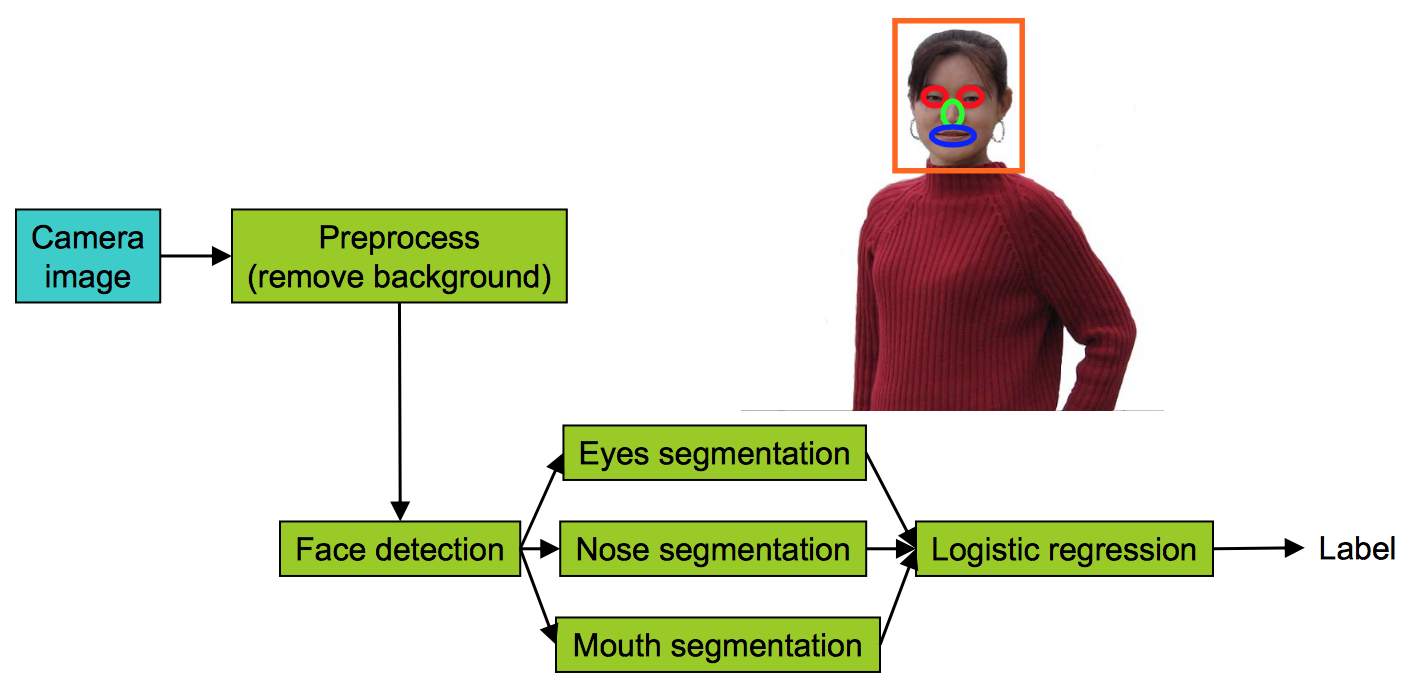
\includegraphics[width=\textwidth]{pipeline.png}
	\caption{Face recognition pipeline}
	\label{pipeline}
\end{figure}

If you biuld a complicated system like this one, you might want to figure out how much error is attributable to each of the components, how good is each of these green boxes. Indeed, if one of these boxes is really problematic, you might want to spend more time trying to improve the performance of that one green box. How do you decide what part to focus on?

One thing we can do is plug in the ground-truth for each component, and see how accuracy changes. Let's say the overall accuracy of the system is 85\% (pretty bad). You can now take your development set and manually give it the perfect background removal, that is, instead of using your background removal algorithm, manually specify the perfect background removal yourself (using photoshop for instance), and look at how much that affect the performance of the overall system.

Now let's say the accuracy only improves by 0.1\%. This gives us an upperbound, that is even if we worked for years on background removal, it wouldn't help our system by more than 0.1\%.

Now let's give the pipeline the perfect face detection by specifying the position of the face manually, see how much we improve the performance, and so on.

The results are specified in the table \ref{error_analysis}.

\begin{table}[h!]
	\centering
	\begin{tabular}{|c|c|}
		\hline
		\textbf{Component} & \textbf{Accuracy} \\
		\hline
		Overall system & 85\% \\
		\hline
		Preprocess (remove background) & 85.1\% \\
		\hline
		Face detection & 91\% \\
		\hline
		Eyes segmentation & 95\% \\
		\hline
		Nose segmentation & 96\% \\
		\hline
		Mouth segmentation & 97\% \\
		\hline
		Logistic regression & 100\% \\
		\hline
	\end{tabular}
	\caption{Accuracy when providing the system with the perfect component}
	\label{error_analysis}
\end{table}

Looking at the table, we know that working on the background removal won't help much. It also tells us where the biggest jumps are. We notice that having an accurate face detection mechanism really improves the performance, and similarly, the eyes really help making the prediction more accurate.

Error analysis is also useful when publishing a paper, since it's a convenient way to analyze the error of an algorithm and explain which parts should be improved.

\subsection*{Ablative analysis}

While error analysis tries to explain the difference between current performance and perfect performance, ablative analysis tries to explain the difference between some baseline (much poorer) performance and current performance.

For instance, suppose you have built a good anti-spam classifier by adding lots of clever features to logistic regression
\begin{itemize}
	\item Spelling correction
	\item Sender host features
	\item Email header features
	\item Email text parser features
	\item Javascript parser
	\item Features from embedded images
\end{itemize}
and your question is: How much did each of these components really help?

In this example, let's say that simple logistic regression without any clever features gets 94\% performance, but when adding these clever features, we get 99.9\% performance. In abaltive analysis, what we do is start from the current level of performance 99.9\%, and slowly take away all of these features to see how it affects performance. The results are provided in table \ref{ablative_analysis}.

When presenting the results in a paper, ablative analysis really helps analyzing the features that helped decreasing the misclassification rate. Instead of simply giving the loss/error rate of the algorithm, we can provide evidence that some specific features are actually more important than others.

\begin{table}[h!]
	\centering
	\begin{tabular}{|c|c|}
		\hline
		\textbf{Component} & \textbf{Accuracy} \\
		\hline
		Overall system & 99.9\% \\
		\hline
		Spelling correction & 99.0\% \\
		\hline
		Sender host features & 98.9\% \\
		\hline
		Email header features & 98.9\% \\
		\hline
		Email text parser features & 95\% \\
		\hline
		Javascript parser & 94.5\% \\
		\hline
		Features from images & 94.0\% \\
		\hline
	\end{tabular}
	\caption{Accuracy when removing feature from logistic regression}
	\label{ablative_analysis}
\end{table}

\subsection*{Analyze your mistakes}

Assume you are given a dataset with pictures of animals, and your goal is to identify pictures of cats that you would eventually send to the members of a community of cat lovers. You notice that there are many pictures of dogs in the original dataset, and wonders whether you should build a special algorithm to identify the pictures of dogs and avoid sending dogs pictures to cat lovers or not.

One thing you can do is take a 100 examples from your development set that are misclassified, and count up how many of these 100 mistakes are dogs. If 5\% of them are dogs, then even if you come up with a solution to identidy your dogs, your error would only go down by 5\%, that is your accuracy would go up from 90\% to 90.5\%. However, if 50 of these 100 errors are dogs, then you could improve your accuracy to reach 95\%.

By analyzing your mistakes, you can focus on what's really important. If you notice that 80 out of your 100 mistakes are blurry images, then work hard on classifying correctly these blurry images. If you notice that 70 out of the 100 errors are great cats, then focus on this specific task of identifying great cats.

In brief, do not waste your time improving parts of your algorithm that won't really help decreasing your error rate, and focus on what really matters.

\end{document}
